%%%%%%%%%%%%%%%%%%%%%%%%%%%%%%%%%%%%%%%%%%%%%%%%%%%%%%%%%%%%%%%%%%%%%%%%%%%%%%%%%%
\begin{frame}[fragile]\frametitle{}
\begin{center}
{\Large Samadhi Paad समाधिपाद}
\end{center}
\end{frame}


%%%%%%%%%%%%%%%%%%%%%%%%%%%%%%%%%%%%%%%%%%%%%%%%%%%%%%%%%%%
\begin{frame}[fragile]\frametitle{Introduction}


	\begin{itemize}
	\item Samadhi refers to a blissful state of existence that is believed to be even beyond mind and meditation.
	\item In this chapter, the author describes yoga and then our true nature and then he instructs the means to attain Samadhi. 
	\item Patanjali begins this chapter with a definition of yoga.
	\item He lists the obstacles we may encounter to attaining mental silence. 
	\item But, having overcome such obstacles, he explains what it is like when we have achieved mental silence as well.
	\end{itemize}

\tiny{(Ref: Basic Introduction of Patanjali Yoga Sutras – The Best Knowledge for Yogis - Yoga Moha)}

\end{frame}

%%%%%%%%%%%%%%%%%%%%%%%%%%%%%%%%%%%%%%%%%%%%%%%%%%%%%%%%%%%
\begin{frame}[fragile]\frametitle{Types of Samadhi समाधी}

\begin{center}
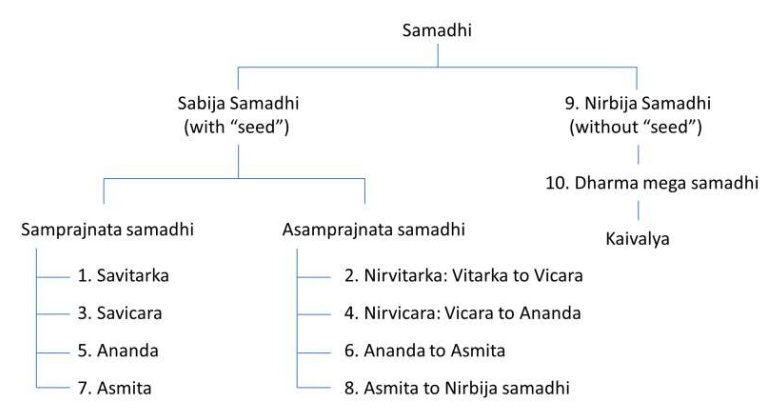
\includegraphics[width=\linewidth,keepaspectratio]{yog37}

\end{center}

  
  \tiny{(Ref: Patanjali Yoga Darshan- For AYUSH YOGA EXAM- Deepak D.Khaire)}

\end{frame}


%%%%%%%%%%%%%%%%%%%%%%%%%%%%%%%%%%%%%%%%%%%%%%%%%%%%%%%%%%%
\begin{frame}[fragile]\frametitle{The Beginning}

अथ योग अनुशासनम् 1.01

	\begin{itemize}
	\item अथ primarily means `now' has many levels of meanings.
	\begin{itemize}
	\item You have done lots of reading, getting knowledge, NOW, lets practice Yog
	\item You have been coming from different evolutionary paths, NOW you are eligible to do Yog
	\item अनुशासनम् means discipline. अनु means following. Now follow the Yog tradition. Meaning Yog was known before (like in Gita), NOW its time to continue/follow it.
	\end{itemize}	
	\end{itemize}

\end{frame}


%%%%%%%%%%%%%%%%%%%%%%%%%%%%%%%%%%%%%%%%%%%%%%%%%%%%%%%%%%%
\begin{frame}[fragile]\frametitle{Definition of Yog}

योग: चित्तवृत्ति निरोध: १.०२

	\begin{itemize}
	\item Yog is complete cessation/stilling of perturbations of mind
	\item चित (chit): to enlighten to know, to make aware (जाणणे/जानना)
	\item चित्त (chitta): the enlightened, all inclusive term, different faculties of mind.
	\item Reality: This is much easier said than done. 
	\item During meditation a cloud of thoughts rolls in like a storm or a swarm of mosquitoes. This can be addressed by acts of observations. \item Awareness itself is our true nature and that the temporary buzz of thoughts, feelings, and sensations is not real or significant. ({\tiny Ref: Rodney Yee Decodes Yoga Sutra 1.2: Calm the Chatter of the Mind})
	\end{itemize}

\end{frame}


%%%%%%%%%%%%%%%%%%%%%%%%%%%%%%%%%%%%%%%%%%%%%%%%%%%%%%%%%%%
\begin{frame}[fragile]\frametitle{चित्त}

	\begin{itemize}
	\item अन्त:करण : मन, बुद्धि, अहंकार, चित्त
	\item Chitta is like a river, flowing in two opposite directions: worldliness to/from Kaivalya कैवल्य (व्यास भाष्य)
	\item Levels of Chitta:
		\begin{itemize}
		\item मूढ चित्त  Dull, intertial, Tamas तमस
		\item क्षिप्त चित्त  Restless, distracted, Rajas  रजस
		\item विक्षिप्त चित्त Sometimes steady Sattva सत्व
		\item एकाग्र चित्त Focused
		\item निरुद्ध चित्त Restricted
		
		\end{itemize}	
	\end{itemize}

\end{frame}

%%%%%%%%%%%%%%%%%%%%%%%%%%%%%%%%%%%%%%%%%%%%%%%%%%%%%%%%%%%
\begin{frame}[fragile]\frametitle{Essence of Yog}

\begin{sanskrit}
योग: चित्तवृत्ति निरोध: १.०२

तदा द्रष्टु: स्वरुपे अवस्थानम् १.०३

वृत्ति सारुप्यं इतरत्र १.०४
\end{sanskrit}


	\begin{itemize}
	\item Yog is complete cessation/stilling of perturbations of mind
	\item Once the stilling happens, Then the seer (Purush, पुरुष ) gets to see his own true nature.
	\item Till that time, there is a continual identification with vruttis वृत्ति like reflection of the moon in the lake.
	\item Essence of Yog: still the mind-lake, to see the true bottom.
	\end{itemize}

\end{frame}

%%%%%%%%%%%%%%%%%%%%%%%%%%%%%%%%%%%%%%%%%%%%%%%%%%%%%%%%%%%
\begin{frame}[fragile]\frametitle{वृत्ति}

	\begin{itemize}
	\item वृत्तय: पञ्चतय्य: क्लिष्टा अक्लिष्टा १.०५
	\item 5 types of vruttis : painful/complicated and not complicated
	\item प्रमाणं विपर्यय विकल्प निद्रा स्मृतय: १.०६
		\begin{itemize}
		\item प्रमाणं : यथार्थ ज्ञान : correct knowledge with right perception
		\item विपर्यय : भ्रामक ज्ञान : False knowledge
		\item विकल्प : काल्पनिक ज्ञान : Imaginary knowledge
		\item निद्रा : अभाव ज्ञान : Lack of knowledge
		\item स्मृति : Memory
		
		\end{itemize}	
	\end{itemize}

\end{frame}

%%%%%%%%%%%%%%%%%%%%%%%%%%%%%%%%%%%%%%%%%%%%%%%%%%%%%%%%%%%
\begin{frame}[fragile]\frametitle{चित्त वृत्ति}

\begin{sanskrit}
प्रत्यक्ष अनुमान आगम: प्रमाणानि १.०७

विपर्यय: मिथ्या ज्ञानम् अतद् रूप प्रतिष्ठम् १.०८

शब्द ज्ञान अनुपाति वस्तु शून्यो विकल्प: १.०९
\end{sanskrit}


	\begin{itemize}
	\item Correct knowledge is obtained through direct perception
	\item Incorrect knowledge is based on false perception, eg rope looks like a snake in the dark
	\item Verbal knowledge which does not have actual object is imaginary knowledge eg horn of rabbit
	\end{itemize}

\end{frame}

%%%%%%%%%%%%%%%%%%%%%%%%%%%%%%%%%%%%%%%%%%%%%%%%%%%%%%%%%%%
\begin{frame}[fragile]\frametitle{Yog}
\begin{sanskrit}
अभावप्रत्ययालम्बना वृत्तिर्निद्रा॥१०॥
\end{sanskrit}
	\begin{itemize}
	\item Yog 
	\end{itemize}
\end{frame}


%%%%%%%%%%%%%%%%%%%%%%%%%%%%%%%%%%%%%%%%%%%%%%%%%%%%%%%%%%%
\begin{frame}[fragile]\frametitle{Yog}
\begin{sanskrit}
अनुभूतविषयासंप्रमोषः स्मृतिः॥११॥
\end{sanskrit}
	\begin{itemize}
	\item Yog 
	\end{itemize}
\end{frame}


%%%%%%%%%%%%%%%%%%%%%%%%%%%%%%%%%%%%%%%%%%%%%%%%%%%%%%%%%%%
\begin{frame}[fragile]\frametitle{Yog}
\begin{sanskrit}
अभ्यासवैराग्याभ्यां तन्निरोधः॥१२॥
\end{sanskrit}
	\begin{itemize}
	\item Yog 
	\end{itemize}
\end{frame}


%%%%%%%%%%%%%%%%%%%%%%%%%%%%%%%%%%%%%%%%%%%%%%%%%%%%%%%%%%%
\begin{frame}[fragile]\frametitle{Yog}
\begin{sanskrit}
तत्र स्थितौ यत्नोऽभ्यासः॥१३॥
\end{sanskrit}
	\begin{itemize}
	\item Yog 
	\end{itemize}
\end{frame}

%%%%%%%%%%%%%%%%%%%%%%%%%%%%%%%%%%%%%%%%%%%%%%%%%%%%%%%%%%%
\begin{frame}[fragile]\frametitle{Yog}
\begin{sanskrit}
स तु दीर्घकालनैरन्तर्यसत्कारासेवितो दृढभूमिः॥१४॥
\end{sanskrit}
	\begin{itemize}
	\item Yog 
	\end{itemize}
\end{frame}

%%%%%%%%%%%%%%%%%%%%%%%%%%%%%%%%%%%%%%%%%%%%%%%%%%%%%%%%%%%
\begin{frame}[fragile]\frametitle{Yog}
\begin{sanskrit}
दृष्टानुश्रविकविषयवितृष्णस्य वशीकारसंज्ञा वैराग्यम्॥१५॥
\end{sanskrit}
	\begin{itemize}
	\item Yog 
	\end{itemize}
\end{frame}


%%%%%%%%%%%%%%%%%%%%%%%%%%%%%%%%%%%%%%%%%%%%%%%%%%%%%%%%%%%
\begin{frame}[fragile]\frametitle{Yog}
\begin{sanskrit}
तत्परं पुरुषख्यातेर्गुणवैतृष्ण्यम्॥१६॥
\end{sanskrit}
	\begin{itemize}
	\item Yog 
	\end{itemize}
\end{frame}



%%%%%%%%%%%%%%%%%%%%%%%%%%%%%%%%%%%%%%%%%%%%%%%%%%%%%%%%%%%
\begin{frame}[fragile]\frametitle{Yog}
\begin{sanskrit}
वितर्कविचारानन्दास्मितारूपानुगमात् संप्रज्ञातः॥१७॥
\end{sanskrit}
	\begin{itemize}
	\item Yog 
	\end{itemize}
\end{frame}

%%%%%%%%%%%%%%%%%%%%%%%%%%%%%%%%%%%%%%%%%%%%%%%%%%%%%%%%%%%
\begin{frame}[fragile]\frametitle{Yog}
\begin{sanskrit}
विरामप्रत्ययाभ्यासपूर्वः संस्कारशेषोऽन्यः॥१८॥
\end{sanskrit}
	\begin{itemize}
	\item Yog 
	\end{itemize}
\end{frame}


%%%%%%%%%%%%%%%%%%%%%%%%%%%%%%%%%%%%%%%%%%%%%%%%%%%%%%%%%%%
\begin{frame}[fragile]\frametitle{Yog}
\begin{sanskrit}
भवप्रत्ययो विदेहप्रकृतिलयानाम्॥१९॥
\end{sanskrit}
	\begin{itemize}
	\item Yog 
	\end{itemize}
\end{frame}

%%%%%%%%%%%%%%%%%%%%%%%%%%%%%%%%%%%%%%%%%%%%%%%%%%%%%%%%%%%
\begin{frame}[fragile]\frametitle{Yog}
\begin{sanskrit}
श्रद्धावीर्यस्मृतिसमाधिप्रज्ञापूर्वक इतरेषाम्॥२०॥
\end{sanskrit}
	\begin{itemize}
	\item Yog 
	\end{itemize}
\end{frame}

%%%%%%%%%%%%%%%%%%%%%%%%%%%%%%%%%%%%%%%%%%%%%%%%%%%%%%%%%%%
\begin{frame}[fragile]\frametitle{Yog}
\begin{sanskrit}
तीव्रसंवेगानामासन्नः॥२१॥
\end{sanskrit}
	\begin{itemize}
	\item Yog 
	\end{itemize}
\end{frame}


%%%%%%%%%%%%%%%%%%%%%%%%%%%%%%%%%%%%%%%%%%%%%%%%%%%%%%%%%%%
\begin{frame}[fragile]\frametitle{Yog}
\begin{sanskrit}
मृदुमध्याधिमात्रत्वात् ततोऽपि विशेषः॥२२॥
\end{sanskrit}
	\begin{itemize}
	\item Yog 
	\end{itemize}
\end{frame}


%%%%%%%%%%%%%%%%%%%%%%%%%%%%%%%%%%%%%%%%%%%%%%%%%%%%%%%%%%%
\begin{frame}[fragile]\frametitle{Yog}
\begin{sanskrit}
ईश्वरप्रणिधानाद्वा॥२३॥
\end{sanskrit}
	\begin{itemize}
	\item Yog 
	\end{itemize}
\end{frame}

%%%%%%%%%%%%%%%%%%%%%%%%%%%%%%%%%%%%%%%%%%%%%%%%%%%%%%%%%%%
\begin{frame}[fragile]\frametitle{Yog}
\begin{sanskrit}
क्लेशकर्मविपाकाशयैरपरामृष्टः पुरुषविशेष ईश्वरः॥२४॥
\end{sanskrit}
	\begin{itemize}
	\item Yog 
	\end{itemize}
\end{frame}

%%%%%%%%%%%%%%%%%%%%%%%%%%%%%%%%%%%%%%%%%%%%%%%%%%%%%%%%%%%
\begin{frame}[fragile]\frametitle{Yog}
\begin{sanskrit}
तत्र निरतिशयं सर्वज्ञबीजम्॥२५॥
\end{sanskrit}
	\begin{itemize}
	\item Yog 
	\end{itemize}
\end{frame}

%%%%%%%%%%%%%%%%%%%%%%%%%%%%%%%%%%%%%%%%%%%%%%%%%%%%%%%%%%%
\begin{frame}[fragile]\frametitle{Yog}
\begin{sanskrit}
पूर्वेषाम् अपि गुरुः कालेनानवच्छेदात्॥२६॥
\end{sanskrit}
	\begin{itemize}
	\item Yog 
	\end{itemize}
\end{frame}

%%%%%%%%%%%%%%%%%%%%%%%%%%%%%%%%%%%%%%%%%%%%%%%%%%%%%%%%%%%
\begin{frame}[fragile]\frametitle{Yog}
\begin{sanskrit}
तस्य वाचकः प्रणवः॥२७॥
\end{sanskrit}
	\begin{itemize}
	\item Yog 
	\end{itemize}
\end{frame}


%%%%%%%%%%%%%%%%%%%%%%%%%%%%%%%%%%%%%%%%%%%%%%%%%%%%%%%%%%%
\begin{frame}[fragile]\frametitle{Yog}
\begin{sanskrit}
तज्जपस्तदर्थभावनम्॥२८॥
\end{sanskrit}
	\begin{itemize}
	\item Yog 
	\end{itemize}
\end{frame}


%%%%%%%%%%%%%%%%%%%%%%%%%%%%%%%%%%%%%%%%%%%%%%%%%%%%%%%%%%%
\begin{frame}[fragile]\frametitle{Yog}
\begin{sanskrit}
ततः प्रत्यक्चेतनाधिगमोऽप्यन्तरायाभावश्च॥२९॥
\end{sanskrit}
	\begin{itemize}
	\item Yog 
	\end{itemize}
\end{frame}




%%%%%%%%%%%%%%%%%%%%%%%%%%%%%%%%%%%%%%%%%%%%%%%%%%%%%%%%%%%
\begin{frame}[fragile]\frametitle{Yog}
\begin{sanskrit}
व्याधिस्त्यानसंशयप्रमादालस्याविरतिभ्रान्तिदर्शनालब्धभूमिकत्वानवस्थितत्वानि चित्तविक्षेपास्तेऽन्तरायाः॥३०॥
\end{sanskrit}
	\begin{itemize}
	\item Yog 
	\end{itemize}
\end{frame}




%%%%%%%%%%%%%%%%%%%%%%%%%%%%%%%%%%%%%%%%%%%%%%%%%%%%%%%%%%%
\begin{frame}[fragile]\frametitle{Yog}
\begin{sanskrit}
दुःखदौर्मनस्याङ्गमेजयत्वश्वासप्रश्वासा विक्षेपसहभुवः॥३१॥
\end{sanskrit}
	\begin{itemize}
	\item Yog 
	\end{itemize}
\end{frame}



%%%%%%%%%%%%%%%%%%%%%%%%%%%%%%%%%%%%%%%%%%%%%%%%%%%%%%%%%%%
\begin{frame}[fragile]\frametitle{Yog}
\begin{sanskrit}
तत्प्रतिषेधार्थमेकतत्त्वाभ्यासः॥३२॥
\end{sanskrit}
	\begin{itemize}
	\item Yog 
	\end{itemize}
\end{frame}



%%%%%%%%%%%%%%%%%%%%%%%%%%%%%%%%%%%%%%%%%%%%%%%%%%%%%%%%%%%
\begin{frame}[fragile]\frametitle{Yog}
\begin{sanskrit}
मैत्रीकरुणामुदितोपेक्षणां सुखदुःखपुण्यापुण्यविषयाणां भावनातश्चित्तप्रसादनम्॥३३॥
\end{sanskrit}
	\begin{itemize}
	\item Yog 
	\end{itemize}
\end{frame}


%%%%%%%%%%%%%%%%%%%%%%%%%%%%%%%%%%%%%%%%%%%%%%%%%%%%%%%%%%%
\begin{frame}[fragile]\frametitle{Yog}
\begin{sanskrit}
प्रच्छर्दनविधारणाभ्यां वा प्राणस्य॥३४॥
\end{sanskrit}
	\begin{itemize}
	\item Yog 
	\end{itemize}
\end{frame}


%%%%%%%%%%%%%%%%%%%%%%%%%%%%%%%%%%%%%%%%%%%%%%%%%%%%%%%%%%%
\begin{frame}[fragile]\frametitle{Yog}
\begin{sanskrit}
विषयवती वा प्रवृत्तिरुत्पन्ना मनसः स्थितिनिबन्धिनी॥३५॥
\end{sanskrit}
	\begin{itemize}
	\item Yog 
	\end{itemize}
\end{frame}




%%%%%%%%%%%%%%%%%%%%%%%%%%%%%%%%%%%%%%%%%%%%%%%%%%%%%%%%%%%
\begin{frame}[fragile]\frametitle{Yog}
\begin{sanskrit}
विशोका वा ज्योतिष्मती॥३६॥
\end{sanskrit}
	\begin{itemize}
	\item Yog 
	\end{itemize}
\end{frame}




%%%%%%%%%%%%%%%%%%%%%%%%%%%%%%%%%%%%%%%%%%%%%%%%%%%%%%%%%%%
\begin{frame}[fragile]\frametitle{Yog}
\begin{sanskrit}
वीतरागविषयं वा चित्तम्॥३७॥
\end{sanskrit}
	\begin{itemize}
	\item Yog 
	\end{itemize}
\end{frame}


%%%%%%%%%%%%%%%%%%%%%%%%%%%%%%%%%%%%%%%%%%%%%%%%%%%%%%%%%%%
\begin{frame}[fragile]\frametitle{Yog}
\begin{sanskrit}
स्वप्ननिद्राज्ञानालम्बनं वा॥३८॥
\end{sanskrit}
	\begin{itemize}
	\item Yog 
	\end{itemize}
\end{frame}



%%%%%%%%%%%%%%%%%%%%%%%%%%%%%%%%%%%%%%%%%%%%%%%%%%%%%%%%%%%
\begin{frame}[fragile]\frametitle{Yog}
\begin{sanskrit}
यथाभिमतध्यानाद्व॥३९॥
\end{sanskrit}
	\begin{itemize}
	\item Yog 
	\end{itemize}
\end{frame}




%%%%%%%%%%%%%%%%%%%%%%%%%%%%%%%%%%%%%%%%%%%%%%%%%%%%%%%%%%%
\begin{frame}[fragile]\frametitle{Yog}
\begin{sanskrit}
परमाणु परममहत्त्वान्तोऽस्य वशीकारः॥४०॥
\end{sanskrit}
	\begin{itemize}
	\item Yog 
	\end{itemize}
\end{frame}

%%%%%%%%%%%%%%%%%%%%%%%%%%%%%%%%%%%%%%%%%%%%%%%%%%%%%%%%%%%
\begin{frame}[fragile]\frametitle{Yog}
\begin{sanskrit}
क्षीणवृत्तेरभिजातस्येव मणेर्ग्रहीतृग्रहणग्राह्येषु तत्स्थतदञ्जनतासमापत्तिः॥४१॥
\end{sanskrit}
	\begin{itemize}
	\item Yog 
	\end{itemize}
\end{frame}

%%%%%%%%%%%%%%%%%%%%%%%%%%%%%%%%%%%%%%%%%%%%%%%%%%%%%%%%%%%
\begin{frame}[fragile]\frametitle{Yog}
\begin{sanskrit}
तत्र शब्दार्थज्ञानविकल्पैः संकीर्णा सवितर्का समापत्तिः॥४२॥
\end{sanskrit}
	\begin{itemize}
	\item Yog 
	\end{itemize}
\end{frame}


%%%%%%%%%%%%%%%%%%%%%%%%%%%%%%%%%%%%%%%%%%%%%%%%%%%%%%%%%%%
\begin{frame}[fragile]\frametitle{Yog}
\begin{sanskrit}
स्मृतिपरिशुद्धौ स्वरूपशून्येवार्थमात्रनिर्भासा निर्वितर्का॥४३॥
\end{sanskrit}
	\begin{itemize}
	\item Yog 
	\end{itemize}
\end{frame}


%%%%%%%%%%%%%%%%%%%%%%%%%%%%%%%%%%%%%%%%%%%%%%%%%%%%%%%%%%%
\begin{frame}[fragile]\frametitle{Yog}
\begin{sanskrit}
एतयैव सविचारा निर्विचारा च सूक्ष्मविषया व्याख्याता॥४४॥
\end{sanskrit}
	\begin{itemize}
	\item Yog 
	\end{itemize}
\end{frame}


%%%%%%%%%%%%%%%%%%%%%%%%%%%%%%%%%%%%%%%%%%%%%%%%%%%%%%%%%%%
\begin{frame}[fragile]\frametitle{Yog}
\begin{sanskrit}
सूक्ष्मविषयत्वं चालिङ्गपर्यवसानम्॥४५॥
\end{sanskrit}
	\begin{itemize}
	\item Yog 
	\end{itemize}
\end{frame}

%%%%%%%%%%%%%%%%%%%%%%%%%%%%%%%%%%%%%%%%%%%%%%%%%%%%%%%%%%%
\begin{frame}[fragile]\frametitle{Yog}
\begin{sanskrit}
ता एव सबीजः समाधिः॥४६॥
\end{sanskrit}
	\begin{itemize}
	\item Yog 
	\end{itemize}
\end{frame}


%%%%%%%%%%%%%%%%%%%%%%%%%%%%%%%%%%%%%%%%%%%%%%%%%%%%%%%%%%%
\begin{frame}[fragile]\frametitle{Yog}
\begin{sanskrit}
निर्विचारवैशारद्येऽध्यात्मप्रसादः॥४७॥
\end{sanskrit}
	\begin{itemize}
	\item Yog 
	\end{itemize}
\end{frame}




%%%%%%%%%%%%%%%%%%%%%%%%%%%%%%%%%%%%%%%%%%%%%%%%%%%%%%%%%%%
\begin{frame}[fragile]\frametitle{Yog}
\begin{sanskrit}
ऋतम्भरा तत्र प्रज्ञा॥४८॥
\end{sanskrit}
	\begin{itemize}
	\item Yog 
	\end{itemize}
\end{frame}



%%%%%%%%%%%%%%%%%%%%%%%%%%%%%%%%%%%%%%%%%%%%%%%%%%%%%%%%%%%
\begin{frame}[fragile]\frametitle{Yog}
\begin{sanskrit}
श्रुतानुमानप्रज्ञाभ्यामन्यविषया विशेषार्थत्वात्॥४९॥
\end{sanskrit}
	\begin{itemize}
	\item Yog 
	\end{itemize}
\end{frame}


%%%%%%%%%%%%%%%%%%%%%%%%%%%%%%%%%%%%%%%%%%%%%%%%%%%%%%%%%%%
\begin{frame}[fragile]\frametitle{Yog}
\begin{sanskrit}
तज्जः संस्कारोऽन्यसंस्कारप्रतिबन्धी॥५०॥
\end{sanskrit}
	\begin{itemize}
	\item Yog 
	\end{itemize}
\end{frame}


%%%%%%%%%%%%%%%%%%%%%%%%%%%%%%%%%%%%%%%%%%%%%%%%%%%%%%%%%%%
\begin{frame}[fragile]\frametitle{Yog}
\begin{sanskrit}
तस्यापि निरोधे सर्वनिरोधान्निर्बीजः समाधिः॥५१॥
\end{sanskrit}
	\begin{itemize}
	\item Yog 
	\end{itemize}
\end{frame}
